\begin{figure}[htb!]
  \begin{subfigure}[b]{0.23\textwidth}
    \centering
    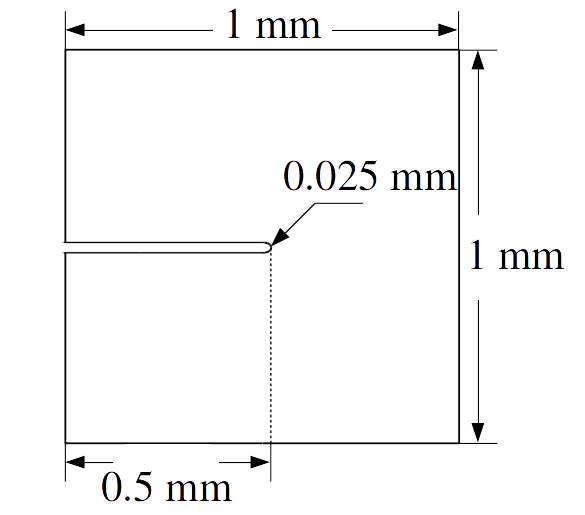
\includegraphics[width=\textwidth,scale=0.5]{Chapter4/figures/notched_plate_dimensions.png}
    \caption{}
    \label{fig: Chapter4/notched_plate_dimensions}
  \end{subfigure}
  \begin{subfigure}[b]{0.21\textwidth}
    \centering
    
\includegraphics[width=\textwidth,scale=0.5]{Chapter4/figures/notched_plate_initial.png}
    \caption{}
    \label{fig: Chapter4/mode1_notched_plate_damage_1}
  \end{subfigure}
  \begin{subfigure}[b]{0.21\textwidth}
    \centering
    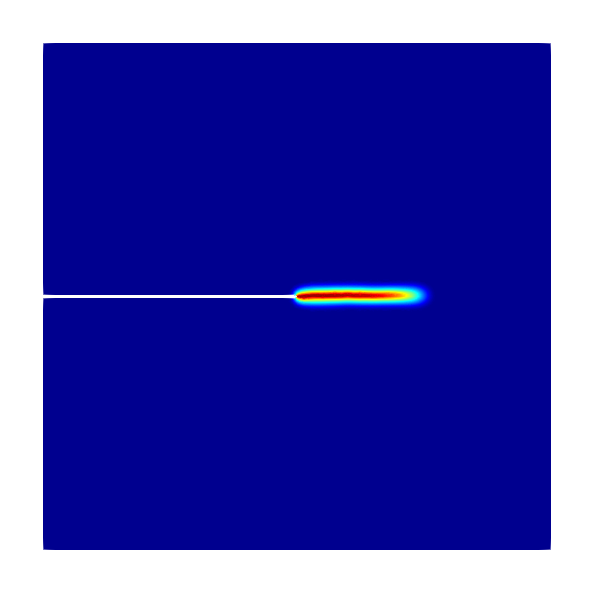
\includegraphics[width=\textwidth,scale=0.5]{Chapter4/figures/mode1_notched_plate_intermediate.png}
    \caption{}
    \label{fig: Chapter4/mode1_notched_plate_damage_2}
  \end{subfigure}
  \begin{subfigure}[b]{0.21\textwidth}
    \centering
    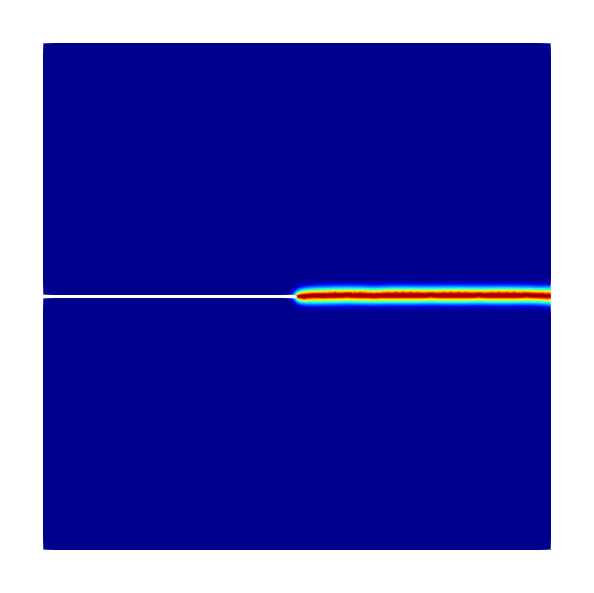
\includegraphics[width=\textwidth,scale=0.5]{Chapter4/figures/mode1_notched_plate_final.png}
    \caption{}
    \label{fig: Chapter4/mode1_notched_plate_damage_3}
  \end{subfigure}
  \begin{subfigure}[b]{0.06\textwidth}
    \centering
    \caption*{d}
    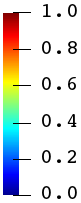
\includegraphics[width=\textwidth]{Chapter4/figures/jet_vertical.png}
    \vspace{0.15in}
  \end{subfigure}
  \caption[Edge-notched specimen loaded in tension with initial crack represented by a geometric notch with a rounded corner.]{Edge-notched specimen loaded in tension with initial crack represented by a geometric notch with a rounded corner.  (a) Dimensions of the notched plate. Damage $d$ at (b) $u_y = \SI{0}{\milli\meter}$, (c) $u_y = \SI{0.0048}{\milli\meter}$, (d) $u_y = \SI{0.006}{\milli\meter}$.}
  \label{fig: Chapter4/mode1_notched_plate}
\end{figure}
